% ============================================================
%  Chapter fragment -- included by main.tex
%  (not a standalone document; compile main.tex to build the PDF)
% ============================================================

\settheme{topic04}
\sheettitle{04 -- PenTesting 1: Security Testing}{SWS2 -- ZHAW / Tellenbach}

% ==================== BIG PICTURE ====================
\section{Security Testing -- Big Picture}

\subsection{4 dimensions}
\begin{itemize}
\item \kw{Why?} find vulns, improve defences, educate/train, compliance, identify attack surface, incident response, improve product security, (unique) selling point.
\item \kw{What?} hardware, app/service, security control, humans, processes, systems, organization, supply chain.
\item \kw{How?} test types: \kw{static / dynamic}, \kw{manual / automated}.
\item \kw{By whom?} internal (devs, security pros), 3rd party, crowd.
\end{itemize}

% ==================== 6 METHODS ====================
\section{6 Security Testing Methods \hl{(!)}}

Each described by: \textit{Purpose, Attacker goal, Assets in scope, Result, Method, Requirement, Frequency.}

\subsection{1. Vulnerability Scanning}
\begin{itemize}
\item Purpose: identify \kw{well-known} vulns; compliance.
\item Scope: source code, apps, systems, whole infra. 
\item Result: \kw{potential} vulns + generic risk rating.
\item Method: \kw{fully automated} (OpenVAS, LGTM).
\item Freq: \kw{continuous} (signatures \& assets change).
\item Req: Needs mature \kw{vuln-management} process (verify/prioritize/fix).
\end{itemize}

\subsection{2. Classical Penetration Testing}
\begin{itemize}
\item Purpose: find as \kw{many vulns as possible} + fixing advice; compliance.
\item Attacker goal: efficiently find many (mainly \kw{"easy-to-find"}) vulns. 
\item Scope: \kw{one/few} (single app/system/service).
\item Result: \kw{verified} vulns + risk rating + fix advice. 
\item Method: (semi-)automated tools + standardized procedures (OWASP guide).
\item Freq: \kw{1--4$\times$/year}, once per new release.
\item Req: Needs mature \kw{vuln-management} process + test environment (e.g. staging with production-like data).
\end{itemize}

\subsection{3. Red-Team Testing}
\begin{itemize}
\item Purpose: test the org's \kw{detection \& response}.
\item Attacker goal: achieve a stated goal \kw{without getting caught} (steal data, become domain admin...). 
\item Scope: \kw{many/all} (physical, human, cyber).
\item Result: goal achieved (y/n) + how. 
\item Method: goal/scope-dependent, often \kw{social engineering}.
\item Req: Needs a \kw{mature security program}. 
\item Freq: periodically(?).
\end{itemize}

\subsection{4. Purple-Team Testing}
\textit{\kw{Blue team} = the defenders (SOC/IR: run monitoring, SIEM, detection rules, respond to incidents). \kw{Security posture} = the org's overall defensive strength -- how well it prevents, detects \& responds to attacks (not just one bug).}
\begin{itemize}
\item Purpose: \kw{improve posture}; focus on \kw{detective/preventive} controls; spot malicious actors already in the environment.
\item \kw{Red + Blue collaborate} (purple = red+blue): attackers \kw{share each move in real time} so defenders learn to detect it.
\item Attacker goal: \kw{help the blue team} catch \& learn from them (not to "win" silently). 
\item Scope: predetermined systems/employees.
\item Result: control improvements (e.g. \kw{new detection rules}) + plan for unresolved gaps. 
\item Method: simulate relevant attack patterns. 
\item Req: Interfaces and collaboration between incident response, security tooling, net engs. and vuln. mngmn. work well
\item Freq: e.g. quarterly.
\end{itemize}

\begin{center}
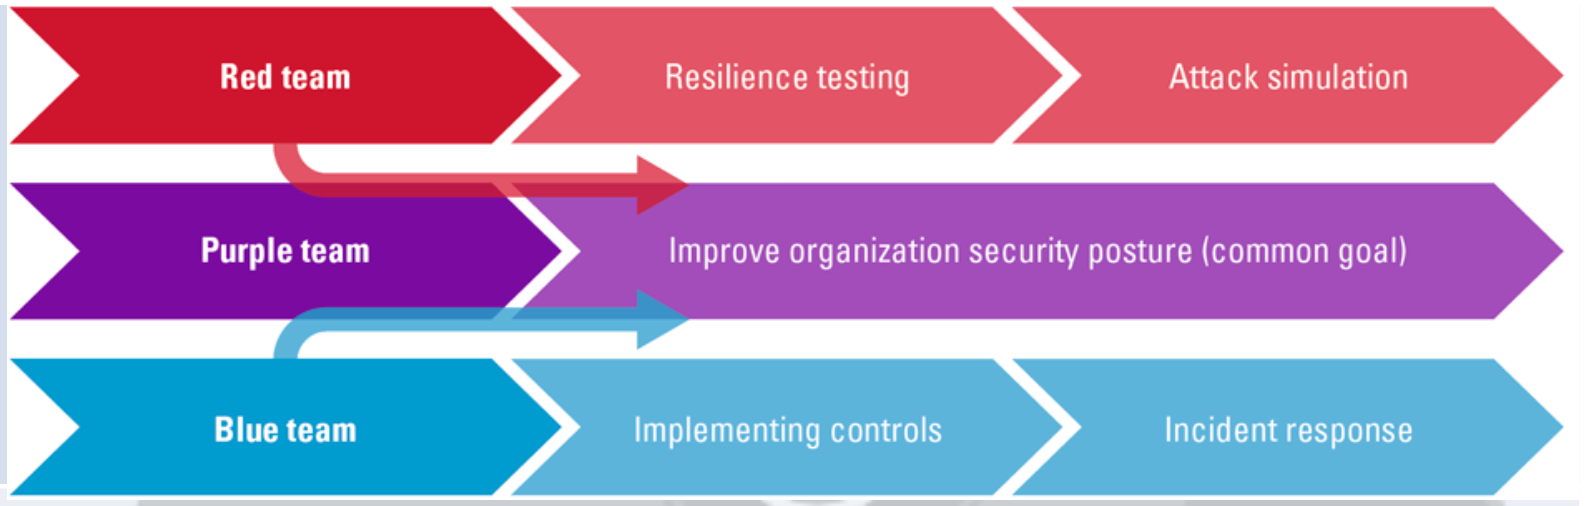
\includegraphics[width=\linewidth]{Figures/purple_team.png}
\end{center}

\subsection{5. Breach \& Attack Simulation}
\begin{itemize}
\item Purpose: improve posture; detective/preventive; uses \kw{prominent attack vectors (MITRE ATT\&CK)}; multi-step along the \kw{kill chain}.
\item Result: resilience report. 
\item Method: \kw{automated platform} (SaaS) running scripted multi-stage attacks. 
\item Freq: \kw{continuous}.
\item Req: Needs purple-team prerequisites + big-budget blue team.
\end{itemize}

\subsection{6. Bug Bounty Program}
\begin{itemize}
\item Purpose: find vulns, \kw{pay only if found}. \kw{Public} (anyone) or \kw{private} (invite only).
\item Attacker goal: earn money/prestige. 
\item Scope: often single app/service. 
\item Result: vuln reports.
\item Method: per program rules (what's allowed). 
\item Req: Needs legal framework + willingness to "go public" + accept \kw{untrusted testers}. 
\item Freq: continuous.
\end{itemize}

\subsection{When to use which}
\begin{center}
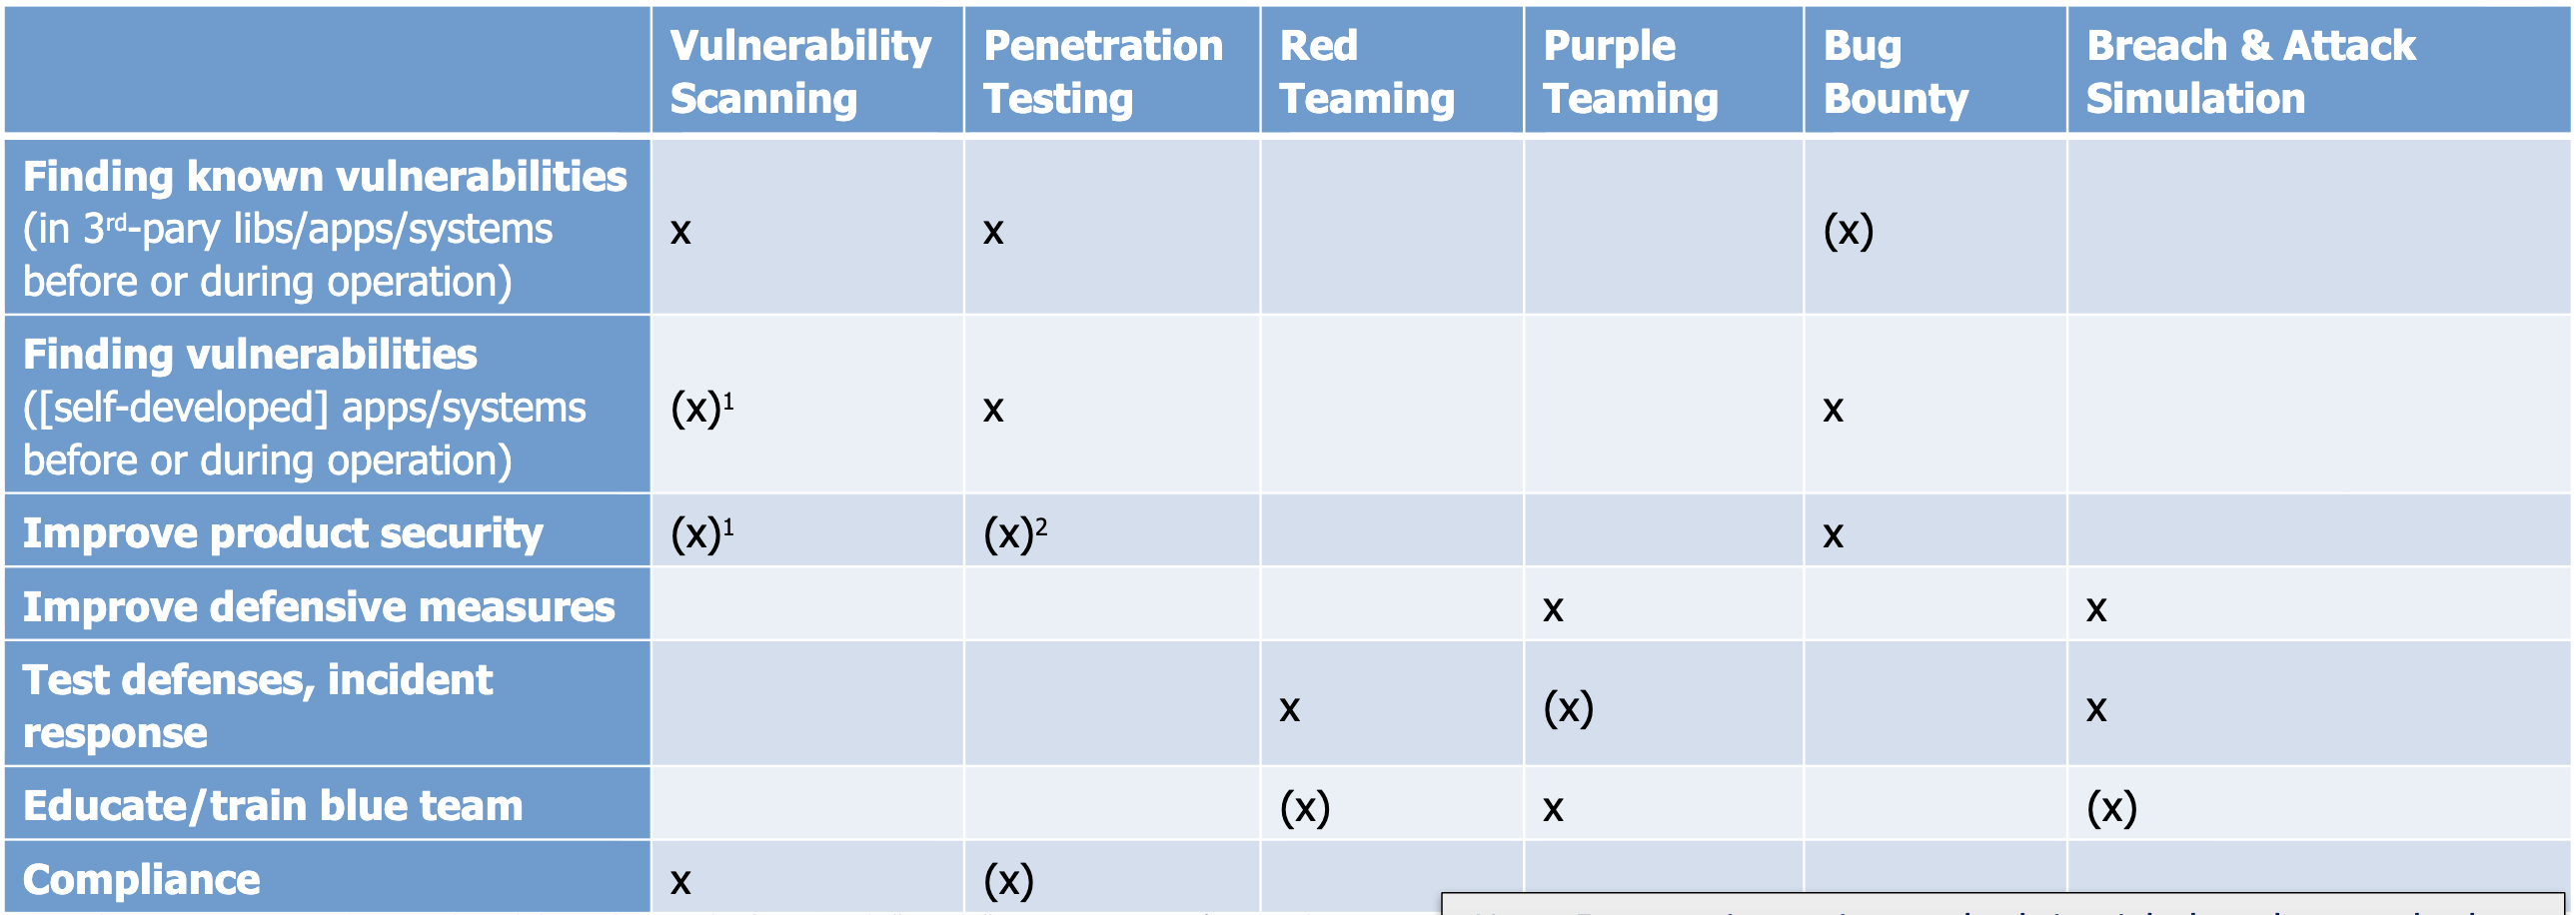
\includegraphics[width=\linewidth]{Figures/when_to_use_which.png}
\end{center}
\textit{Note: matters whether system is internal / public / 3rd-party-hosted (e.g. public bug bounty $\neq$ internal systems).}

% ==================== PENTEST DEFINITION ====================
\section{Penetration Testing}

\subsection{Definition}
\begin{itemize}
\item \kw{NIST SP 800-115}: security testing where assessors \kw{mimic real-world attacks} to find methods of \kw{circumventing security features} of an app/system/network.
\item Business view: analyse all/designated parts of the IT environment to \kw{find \& exploit vulns} and identify the \hl{business risk}.
\end{itemize}
\hl{Caveats:} a pentest is a \kw{snapshot}; "no vuln found" with 1 tester / 10 days / limited gear \kw{proves little}.

\textit{\kw{Is this a pentest?} A Nessus/vuln-scanner report (list of hosts + severities) is \kw{not} a pentest -- that's just a \kw{vulnerability scan}. A pentest \kw{verifies \& exploits} findings and assesses \kw{business risk}.}

\subsection{Motivation}
Find holes \kw{before attackers}; find holes \kw{automated tools can't}; test \kw{detect \& respond}; prove issues to \kw{management}; raise \kw{awareness}; verify configs / new tech; close \kw{compliance} gaps (PCI-DSS, HIPAA).

\subsection{Focus \& scope}
\begin{itemize}
\item Focus on: hacking IT assets, getting \kw{access to info}, physical security, \kw{social engineering}.
\item \kw{Clear but limited scope} (e.g. web-app only from browser's view).
\item Success factors: experience, skills, equipment, \kw{out-of-the-box thinking}.
\end{itemize}

% ==================== METHODOLOGIES ====================
\section{Pentest Methodologies}
\begin{itemize}
\item \kw{OSSTMM} (Open Source Security Testing Methodology Manual): tests \kw{everything} (guards $\to$ satellites); \kw{mathematical model} for a comparable security level.
\item \kw{OWASP Testing Guide} (v4): \kw{web-app} security testing; hands-on advice + tool refs.
\item \kw{NIST SP 800-115}: process (planning, analysis, validation) + Linux-tool appendix.
\item \kw{PTES} (Penetration Testing Execution Standard): basic principles \& steps; industry effort, somewhat outdated/incomplete.
\end{itemize}

% ==================== PHASES ====================
\section{Pentest Phases (PTES) \hl{(!)}}
Cyclic 7 phases:
\begin{itemize}
\item 1 \kw{Pre-engagement Interactions}
\item 2 \kw{Intelligence Gathering}
\item 3 \kw{Threat Modeling}
\item 4 \kw{Vulnerability Analysis}
\item 5 \kw{Exploitation}
\item 6 \kw{Post Exploitation}
\item 7 \kw{Reporting}
\end{itemize}

% ==================== PRE-ENGAGEMENT ====================
\section{Pre-engagement Phase}

\subsection{Three pillars}
\begin{itemize}
\item \kw{Scoping}: define \kw{what} is tested (in-depth single app? over internet w/o employee help? wide IP range to find a way in?).
\item \kw{Rules of Engagement}: \kw{how} testing occurs (method, timeline, locations, evidence handling).
\item \kw{Costs}: estimation; fixed-price vs time \& material.
\end{itemize}

\subsection{Scope -- what does the client want?}
\begin{itemize}
\item Clients often \kw{unaware} of what they need / can't communicate it.
\item Clarify \kw{what} they gain (vulns+risk, fix advice -- or just a checkmark / discredit someone) \& \kw{why} (real problem? compliance? pre-go-live?).
\item Test types: \kw{network, web app, wireless, physical, social engineering}.
\item \kw{Channels} to interact: human, physical, wireless, telecom, data networks.
\item What's included/excluded? 3rd-party assets affected (check \kw{terms of service}, impact on results)? Use \kw{questionnaires/checklists}.
\end{itemize}

\subsection{Rules of Engagement (RoE)}
\begin{itemize}
\item Test method; \kw{timeline}; status meetings (plan/progress/problems).
\item \kw{Time of day} to test (e.g. only 20:00--06:00; don't hit backup 00:00--04:00).
\item Use of \kw{evasion/stealth} (depends on methodology: black/white-box).
\item \hl{Evidence handling}: \kw{encrypt} results, access on \kw{need-to-know}.
\item \hl{Permission-to-test document}: states scope, acknowledges \kw{awareness} of tester activities + \kw{all permissions} (customer, 3rd parties); for online tests $\to$ \kw{liability} waiver if system crashes despite due care.
\end{itemize}

\subsection{Evidence -- sensitive info}
Do \kw{not} store/access \kw{PII}, sensitive PII (religion, race, politics), or \kw{PHI} (health). \textit{But how to prove access was possible without grabbing it?}

\subsection{Communication}
Lines of communication; \kw{emergency contacts} (full name/title, authorization to discuss, 2$\times$ 24/7 contact, secure large-file exchange); incident-reporting process (target \kw{aware} tests are running $\to$ don't wake up mgmt); status report frequency ("ignored customer = former customer"); secure channels.

% ==================== TEST METHODS (OSSTMM) ====================
\section{Test Methods (OSSTMM) \hl{(!)}}
Two axes: \kw{attacker's knowledge of target} vs \kw{target's knowledge of attack}:
\begin{itemize}
\item \kw{Blind}: ethical hacking, war gaming.
\item \kw{Double Blind} = \kw{Black Box} = "classical" pentest (tester knows little, target doesn't know).
\item \kw{Gray Box}: vulnerability test.
\item \kw{Double Gray Box} = \kw{White Box}.
\item \kw{Tandem} = Crystal Box (full mutual knowledge).
\item \kw{Reversal} = Red-Team exercise (tester knows all, target knows nothing).
\end{itemize}
\begin{center}
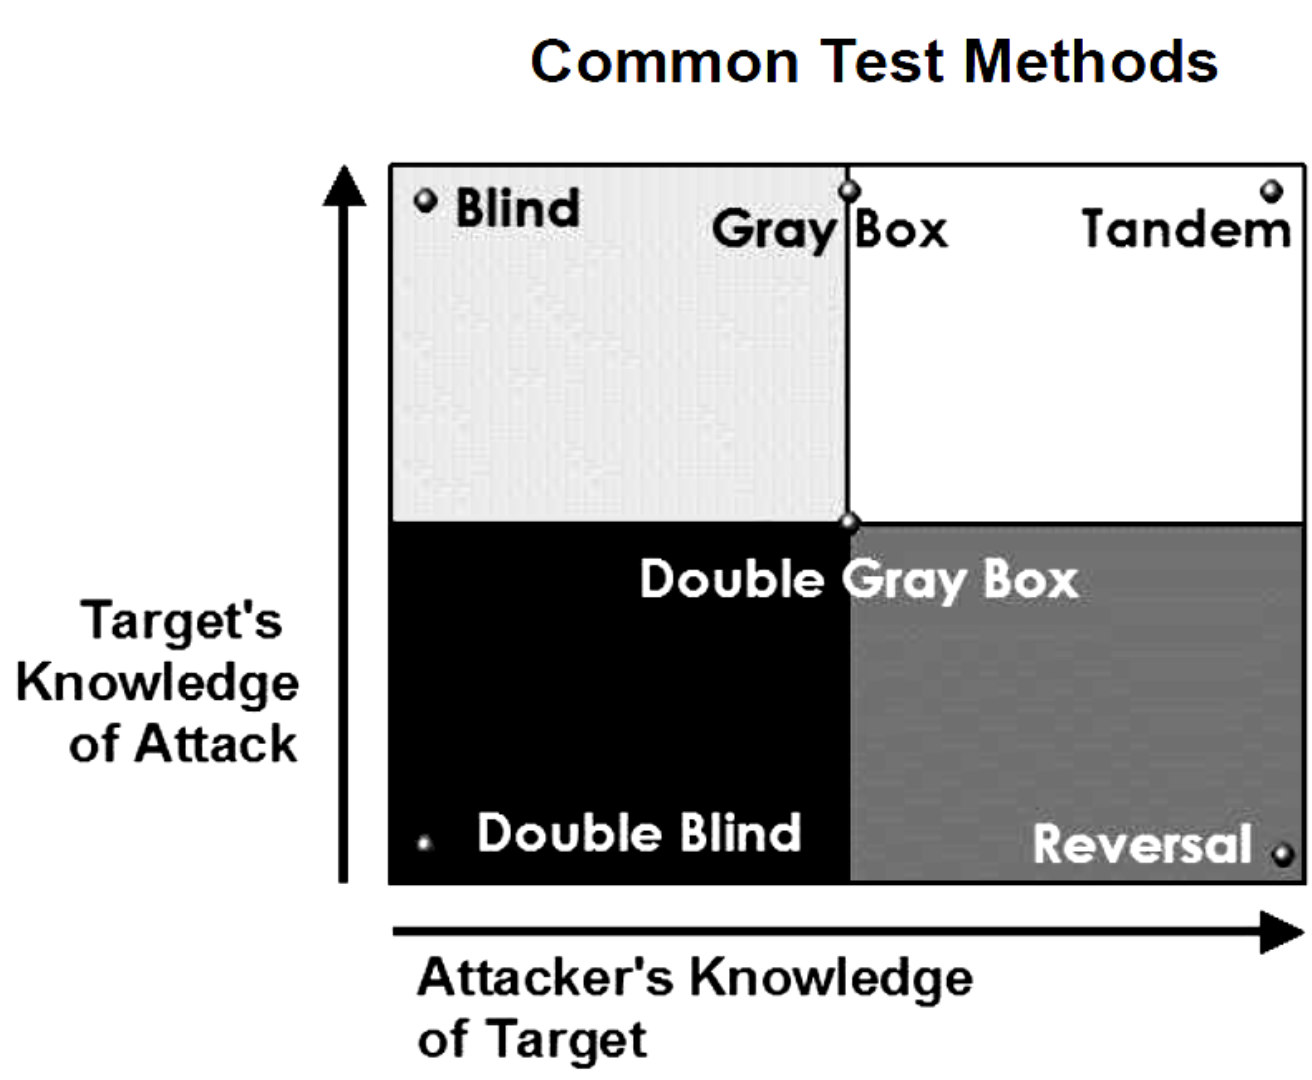
\includegraphics[width=0.5\linewidth]{Figures/common_test_methods.png}
\end{center}

% ==================== CHALLENGE ====================
\section{Challenge -- Scope Creep}
\kw{Scope creep} = extension/alteration of scope needing more time \& effort. \textit{Ex: client asks "please also verify this is exploitable" / "lower the rating from HIGH to MEDIUM".} $\Rightarrow$ stick to scope \& RoE, re-negotiate formally; don't silently expand or falsify ratings.

